\documentclass[11pt]{beamer}
\usepackage[utf8]{inputenc}
\usepackage[T1]{fontenc}
\usepackage{lmodern}
\usepackage[]{babel}
\usepackage{amsmath}
\usepackage{amsfonts}
\usepackage{amssymb}
\usepackage{graphicx}
\usetheme{Madrid}
\DeclareMathOperator*{\argmax}{arg\,max}
\DeclareMathOperator*{\argmin}{arg\,min}

\title{Pricing problems with Thompson Sampling}
\author{Lee Wai Leong Samuel}
\institute{Nanyang Technological University}
\date{23 April 2019}

\AtBeginSection[]
{
\begin{frame}
\frametitle{Table of Contents}
\tableofcontents[currentsection]
\end{frame}
}

\begin{document}

\frame{\titlepage}

\begin{frame}
\frametitle{Table of Contents}
\tableofcontents
\end{frame}

\section{Problem definition}


\begin{frame}
\frametitle{E-commerce trend}
\begin{figure}[h]
\centering
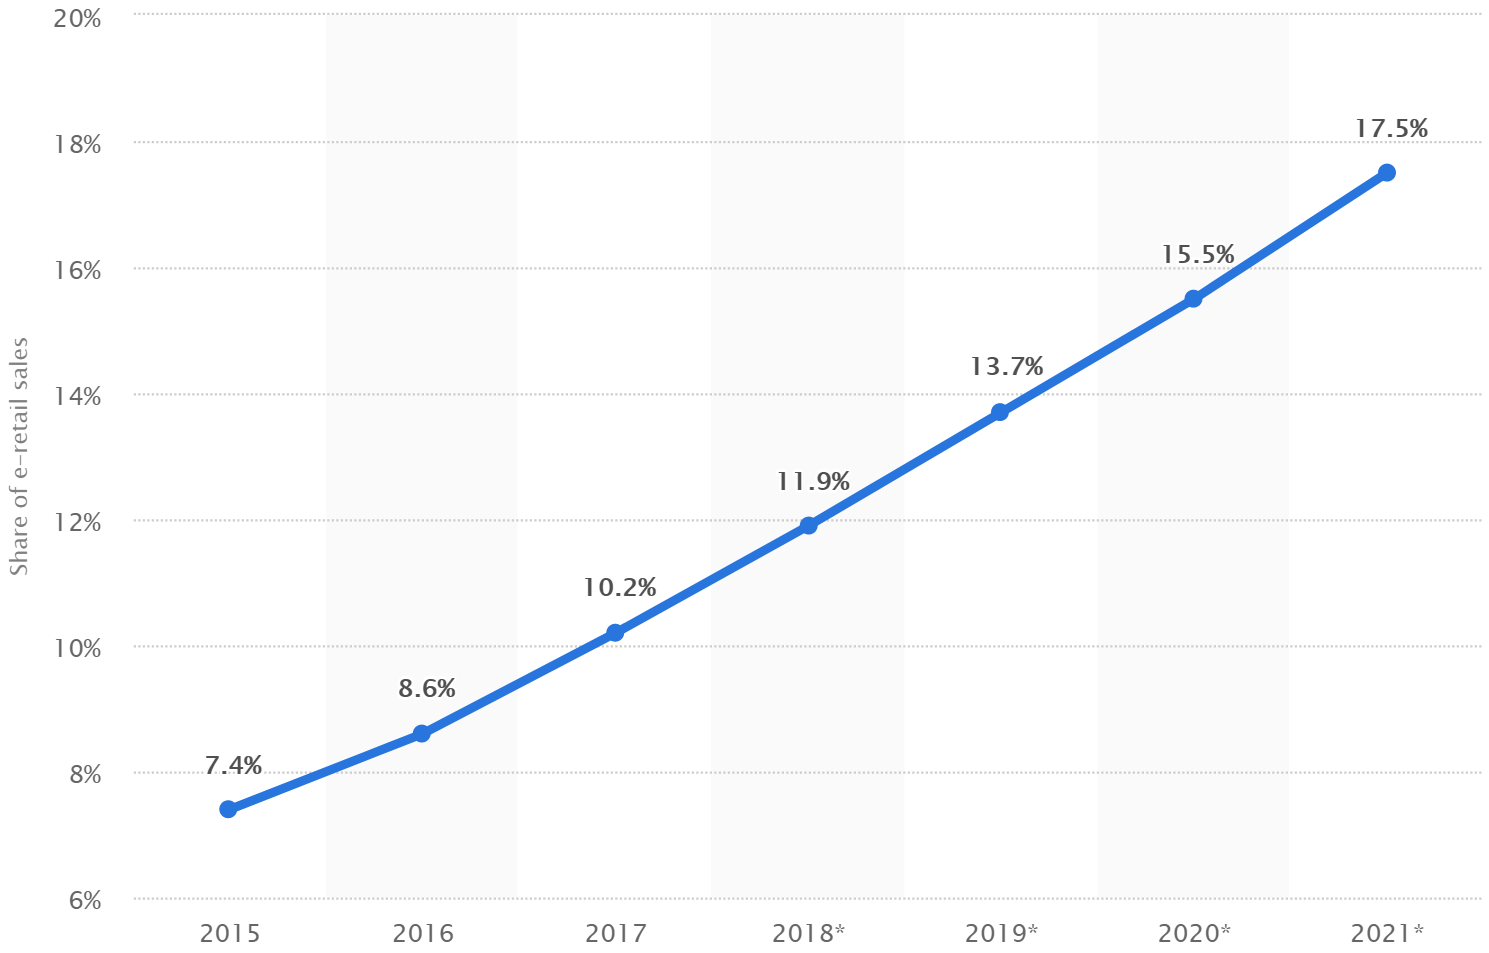
\includegraphics[width=1\textwidth]{statista.png}
\end{figure}
\end{frame}

\begin{frame}
\frametitle{Dynamic Pricing}
\begin{figure}[h]
\centering
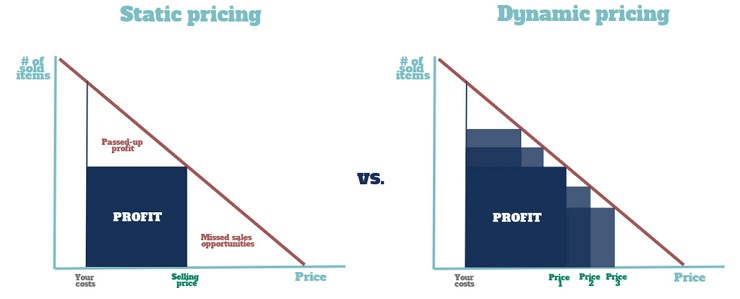
\includegraphics[width=1\textwidth]{dp.jpg}
\end{figure}
\begin{enumerate}
\item Maximise revenue
\item Attract more customers
\item Clear excess inventory
\end{enumerate}
\end{frame}

\begin{frame}
\frametitle{}
\begin{figure}[h]
\centering

\includegraphics[width=0.7\textwidth]{promos.png}
\end{figure}
\centering
We can model dynamic pricing as sales promotions
\end{frame}

\begin{frame}
\frametitle{}
\begin{figure}[h]
\centering
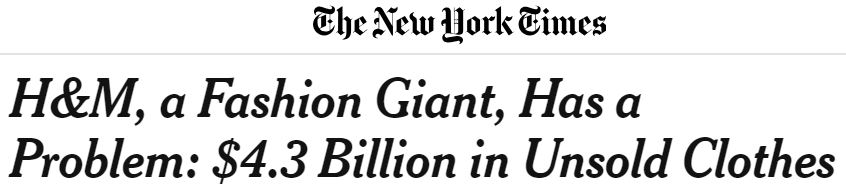
\includegraphics[width=1\textwidth]{hnm.png}
\end{figure}
\begin{figure}[h]
\centering

\includegraphics[width=1\textwidth]{bloomberg.png}
\end{figure}
\begin{figure}[h]
\centering

\includegraphics[width=1\textwidth]{burberry.png}
\end{figure}
\end{frame}

\begin{frame}
\frametitle{}
\begin{figure}[h]
\centering

\includegraphics[width=1\textwidth]{hnm2.png}
\end{figure}
\end{frame}

\section{Classical TS}
\subsection{MNL model}
\subsection{Constant price elasticity model}

\begin{frame}
\frametitle{Why Thompson Sampling?}
Good empirical performance
\begin{enumerate}
\item An Empirical Evaluation of Thompson Sampling (2011). Chapelle, Li
\end{enumerate}
Already extended to revenue management problems
\begin{enumerate}
\item Online Network Revenue Management Using Thompson Sampling (2017). Ferreira, Simchi-Levi, Wang 
\item Thompson Sampling for Complex Online Problems (2014). Gopalan, Mannor, Mansour.
\item Optimization of a SSP’s Header Bidding Strategy using Thompson Sampling (2018). Jauvion, Grislain, Sielenou, Garivier, Gerchinovitz
\item Thompson Sampling for Dynamic Pricing (2018). Ganti, Sustik, Tran, Seaman
\end{enumerate}
\end{frame}

\begin{frame}
\frametitle{Classical Thompson Sampling}
\begin{figure}[h]
\centering

\includegraphics[width=1\textwidth]{mab.png}
\caption{Multi-armed bandit problem}
\end{figure}
Key ideas of Thompson Sampling:
\begin{enumerate}
\item Probability matching
\item Bayesian updating
\end{enumerate}
Pricing problem can be modelled as MAB problem.
\end{frame}

\begin{frame}
\frametitle{MNL model}
Goal: To learn the true demand under each price point
\newline
\newline
Data was created by:
\[X_{ik} = \frac{e^{V_i - P_{ik}}}{\sum_{j=0}^{N}e^{V_j - P_{jk}}}\]
\begin{enumerate}
\item Fixed $V_i$
\item Assumed true demand follows a Normal distribution
\item Created historical data for each of the 3 price points
\item Initialised prior distributions for each price point using MLE
\item Choose a price point and observe $X_{ik}$
\item Add observation to historical data and update distribution
\end{enumerate}

\end{frame}

\begin{frame}
\frametitle{MNL model}
\begin{figure}[h]
\centering
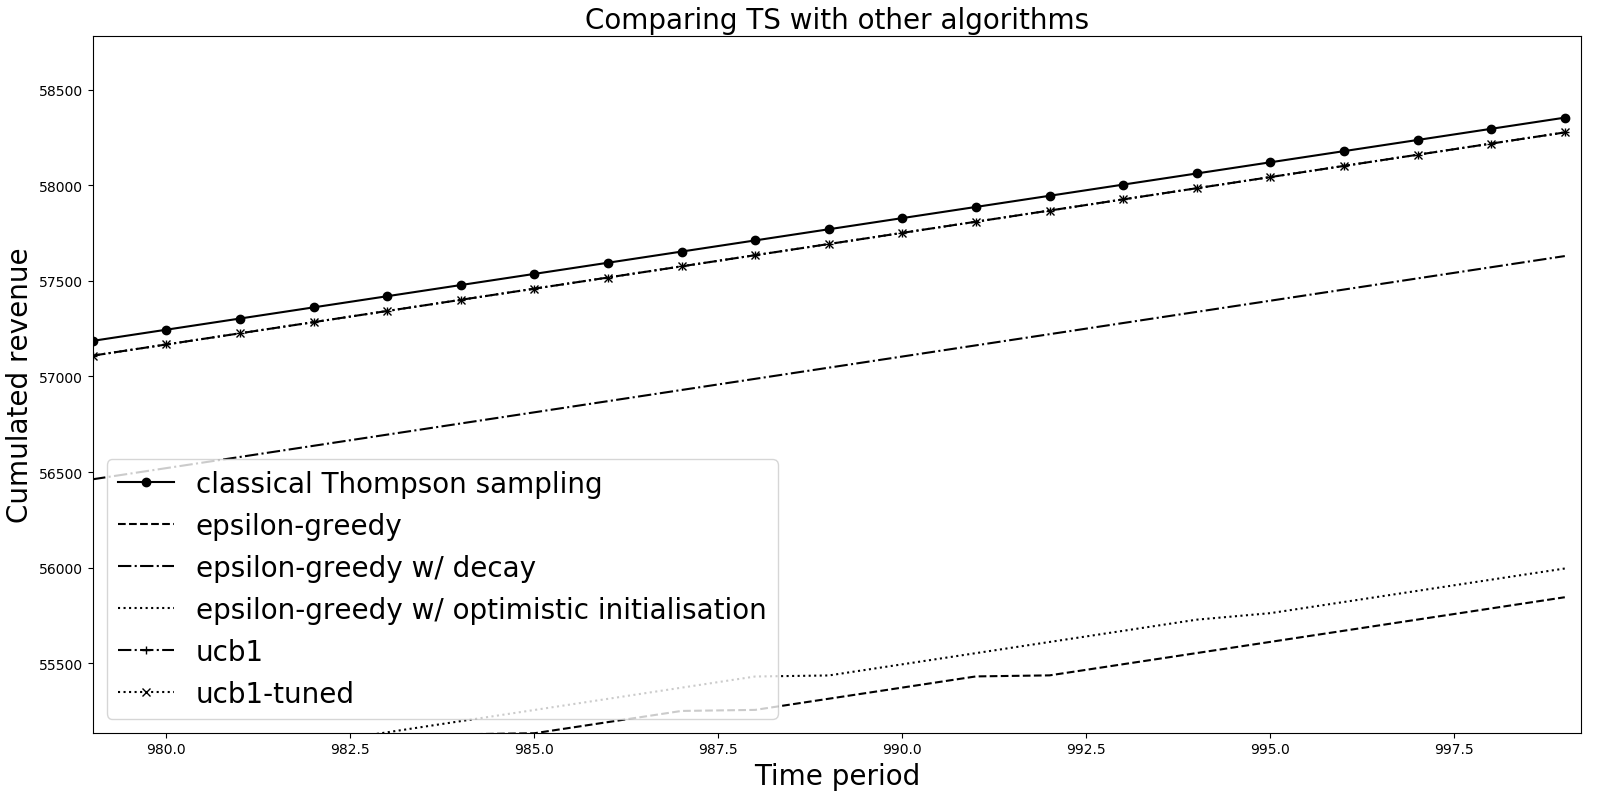
\includegraphics[width=1\textwidth]{Figure_1-4.png}
\caption{\label{fig:three}Comparing revenue between all algorithms (MNL model)}
\end{figure}
\end{frame}

\begin{frame}
\frametitle{Constant price elasticity model}
Goal: To learn the true demand under each price point
\newline
\newline
Data was created by:
\[d_i(p_i) = f_i \left(\frac{p_i}{p_{0,i}}\right)^{\gamma_{*,i}} \]
\begin{enumerate}
\item Fixed $\gamma_{*,i}, f_i, p_{0,i}$ as baseline demand using data from dataset
\item Assumed true demand follows a Normal distribution
\item Created historical data for each of the 3 price points
\item Initialised prior distributions for each price point using MLE
\item Choose a price point and observe $d_i(p_i)$
\item Add observation to historical data and update distribution
\end{enumerate}
\end{frame}

\begin{frame}
\frametitle{Constant price elasticity model}
\begin{figure}[h]
\centering
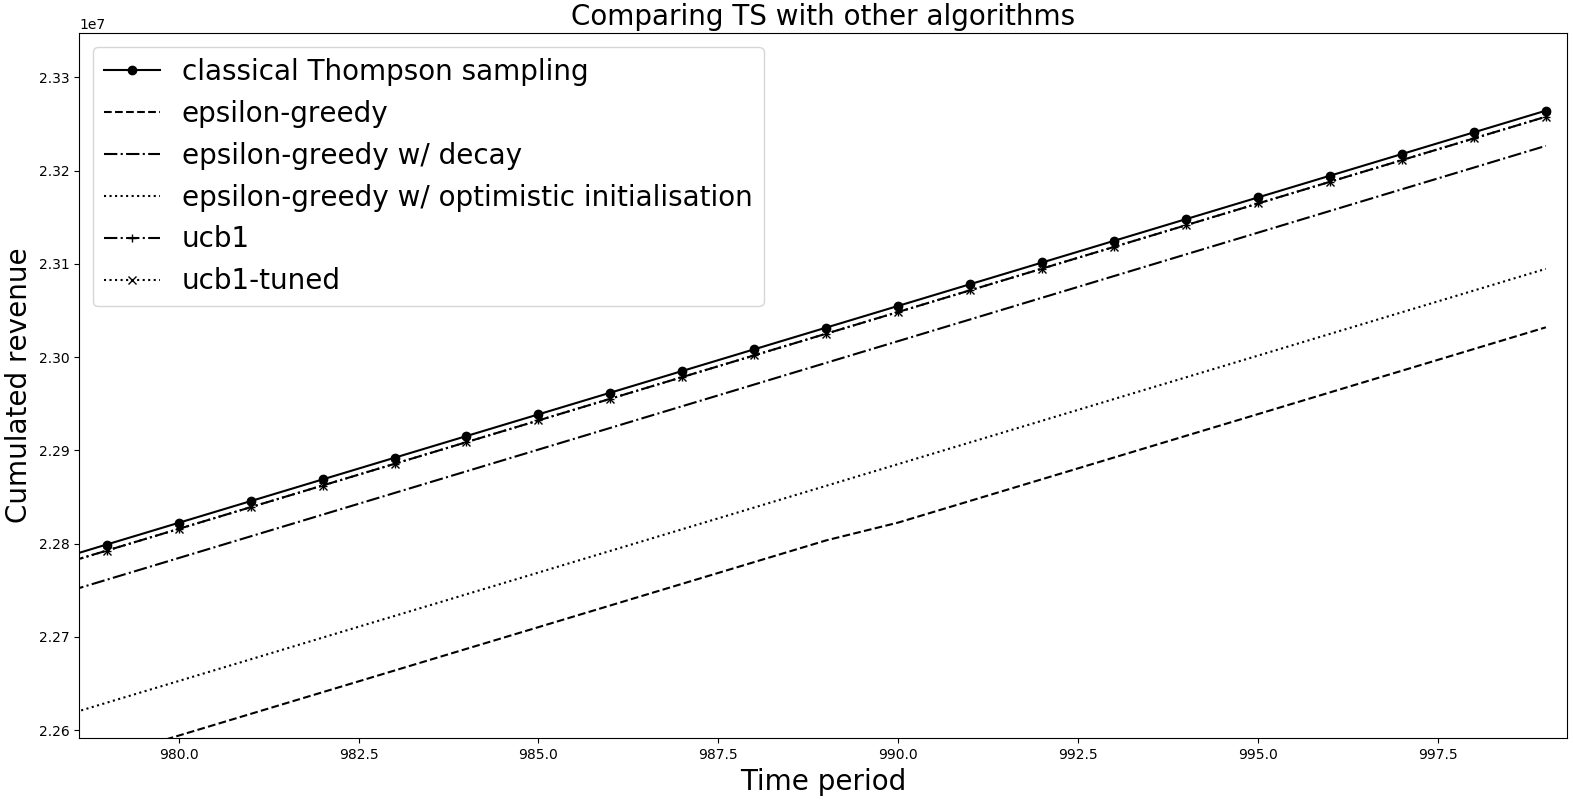
\includegraphics[width=1\textwidth]{6-2.png}
\caption{Comparing revenue between all algorithms (constant elasticity model)}
\end{figure}
\end{frame}

\section{Adapted TS}
\subsection{Non-stationary model}
\subsection{Stationary model}

\begin{frame}
\frametitle{Adapted TS}
Proposed by Ganti, Sustik, Tran, Seaman in Thompson Sampling for Dynamic Pricing (2018).
\newline
\newline
Goal: To learn elasticity $\gamma_*$ instead of demand
\begin{enumerate}
\item Place a prior distribution on $\gamma_t \sim N(\mu, \Sigma)$
\item Sample from $\gamma_t$ until all components are negative
\item Use a time series model to forecast demand $f_{i,t}$ 
\item Solve the optimisation problem to obtain new prices $p_t = \argmax_p  \sum_{i=1}^{N}\frac{p_i^2f_{i,t}\gamma_{*,i}}{p_{i,t-1}} -p_if_{i,t}\gamma_{*,i} + p_if_{i,t}$
\item Apply prices $p_t$ and observe reward
\item Update distribution of $\gamma_t$
\end{enumerate}
\end{frame}

\begin{frame}
\frametitle{Adapted TS}
Goal: To learn elasticity $\gamma_*$ instead of demand
\newline
Non-stationary demand model:
\[d_{i,t}(p_i) = f_{i,t} \left(\frac{p_i}{p_{i,t-1}}\right)^{\gamma_{*,i}} \]
\begin{enumerate}
	\item Used auto regressive model $ f_{i,t} = 0.05 + \sum_{\tau=t-1}^{0} 0.5^{t-\tau}d_{i,\tau} + \epsilon_t $
	\item Fixed $\gamma_{*,i}, d_{i,0}$ as baseline demand using data from dataset
	\item Random initialisation of parameters for prior distribution $\gamma_t$
\end{enumerate}
Stationary demand model:
\[d_i(p_i) = f_i \left(\frac{p_i}{p_{0,i}}\right)^{\gamma_{*,i}} \]
\begin{enumerate}
\item Fixed $\gamma_{*,i}, f_i, p_{0,i}$ as baseline demand using data from dataset
\item Random initialisation of parameters for prior distribution $\gamma_t$
\end{enumerate}
\end{frame}

\begin{frame}
\frametitle{With inventory constraints}
\begin{figure}[h]
\centering
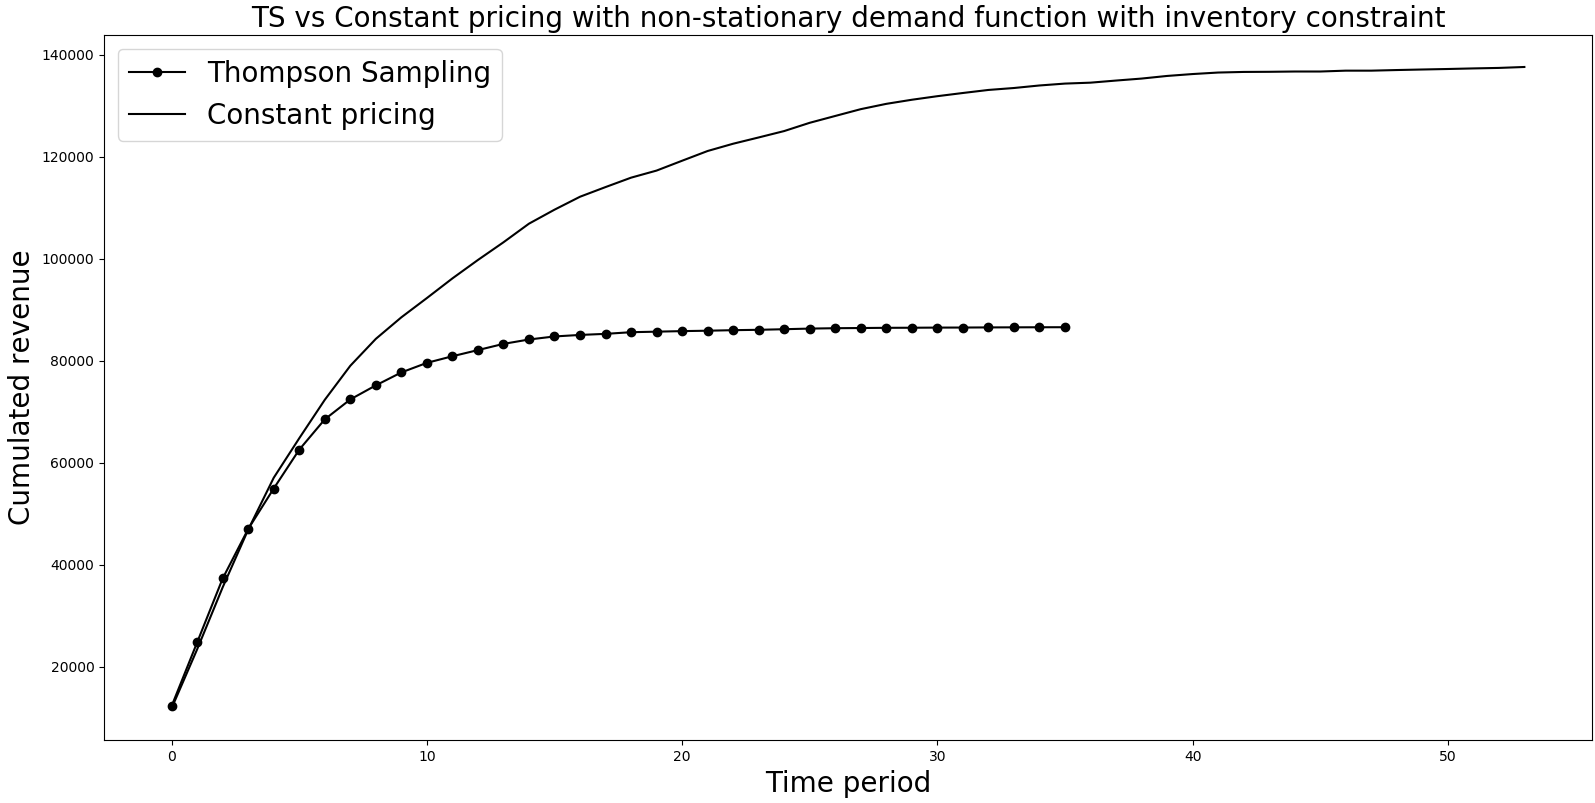
\includegraphics[width=1\textwidth]{4.png}
\caption{\label{fig:five}Cumulated revenue of TS and constant pricing with inventory constraints}
\end{figure}
\end{frame}

\begin{frame}
\frametitle{Without inventory constraints}
\begin{figure}[h]
\centering
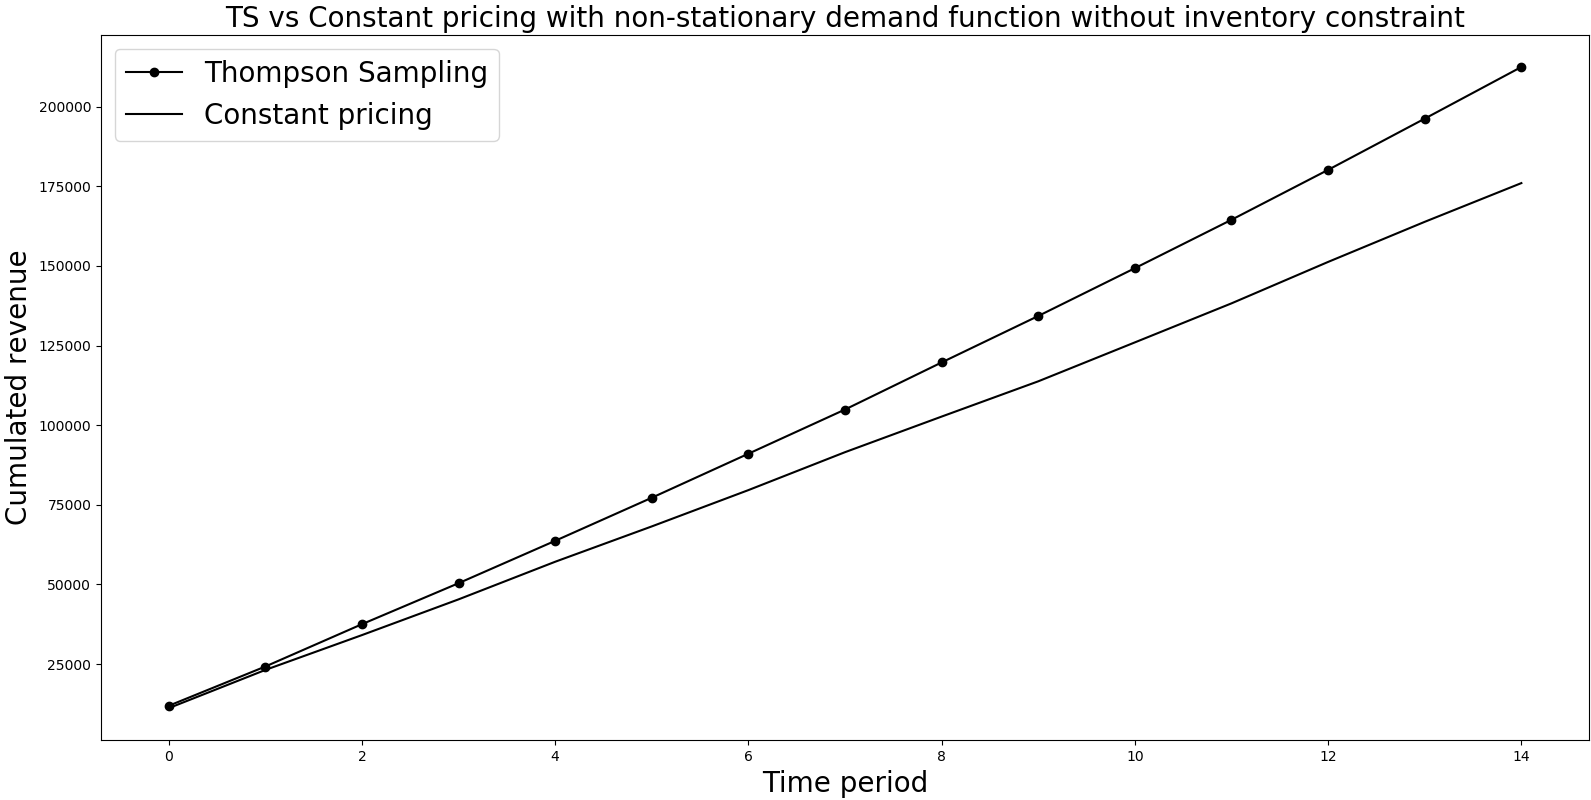
\includegraphics[width=1\textwidth]{2.png}
\caption{\label{fig:four}Cumulated revenue between TS and constant pricing without inventory constraints}
\end{figure}
\end{frame}

\begin{frame}
\frametitle{Conclusion}
\begin{itemize}
	\item Thompson sampling may work just as well as if not better than commonly used algorithms if given good priors
	\item Dynamic Thompson sampling works best if inventory constraints are not a concern
	\item When Thompson sampling works well, it helps with maximising revenue and clearing inventory
\end{itemize}
\end{frame}

\begin{frame}
\frametitle{References}
\begin{itemize}
\item https://www.doofinder.com/en/blog/what-is-e-commerce
\item https://www.cleverism.com/complete-guide-dynamic-pricing/
\item https://www.nytimes.com/2018/03/27/business/hm-clothes-stock-sales.html
\item https://www.nytimes.com/2018/09/06/business/burberry-burning-unsold-stock.html
\item https://www.nytimes.com/reuters/2019/04/17/business/17reuters-h-m-strategy-ai.html
\item https://www.bloomberg.com/news/articles/2017-11-24/burning-h-m-rags-is-new-black-as-swedish-plant-ditches-coal
\item https://imscdrmba.wordpress.com/integrated-marketing-communication/unit-iii-sales-promotion/
\item An Empirical Evaluation of Thompson Sampling (2011). Chapelle, Li
\item Online Network Revenue Management Using Thompson Sampling (2017). Ferreira, Simchi-Levi, Wang 
\item Thompson Sampling for Complex Online Problems (2014). Gopalan, Mannor, Mansour.
\end{itemize}
\end{frame}

\begin{frame}
\frametitle{References}
\begin{itemize}
\item Optimization of a SSP’s Header Bidding Strategy using Thompson Sampling (2018). Jauvion, Grislain, Sielenou, Garivier, Gerchinovitz
\item Thompson Sampling for Dynamic Pricing (2018). Ganti, Sustik, Tran, Seaman
\end{itemize}
\end{frame}

\end{document}
